\subsection{22 августа. Д.р. Джалпаккол}
\textit{Метеоусловия: утром, днём ясно, вечером~--- переменная облачность, тепло. Ночью сильная гроза.}

Из-за позднего завершения ходового дня накануне устраиваем подъём достаточно поздно, в 08:00, и выходим в 10:00. Движемся по правому берегу р. Джалпаккол, не переходя на левый берег у коша N 43.296700\degree,~E 42.046662\degree. Тропа хорошо наибита, место часто посещаемо: обогнали группу пенсионеров, поднимавшихся от т/б <<Глобус>> к водопадам д.р. Кичкинекол Джалпаккольский.

\begin{figure}[h!]
	\centering
	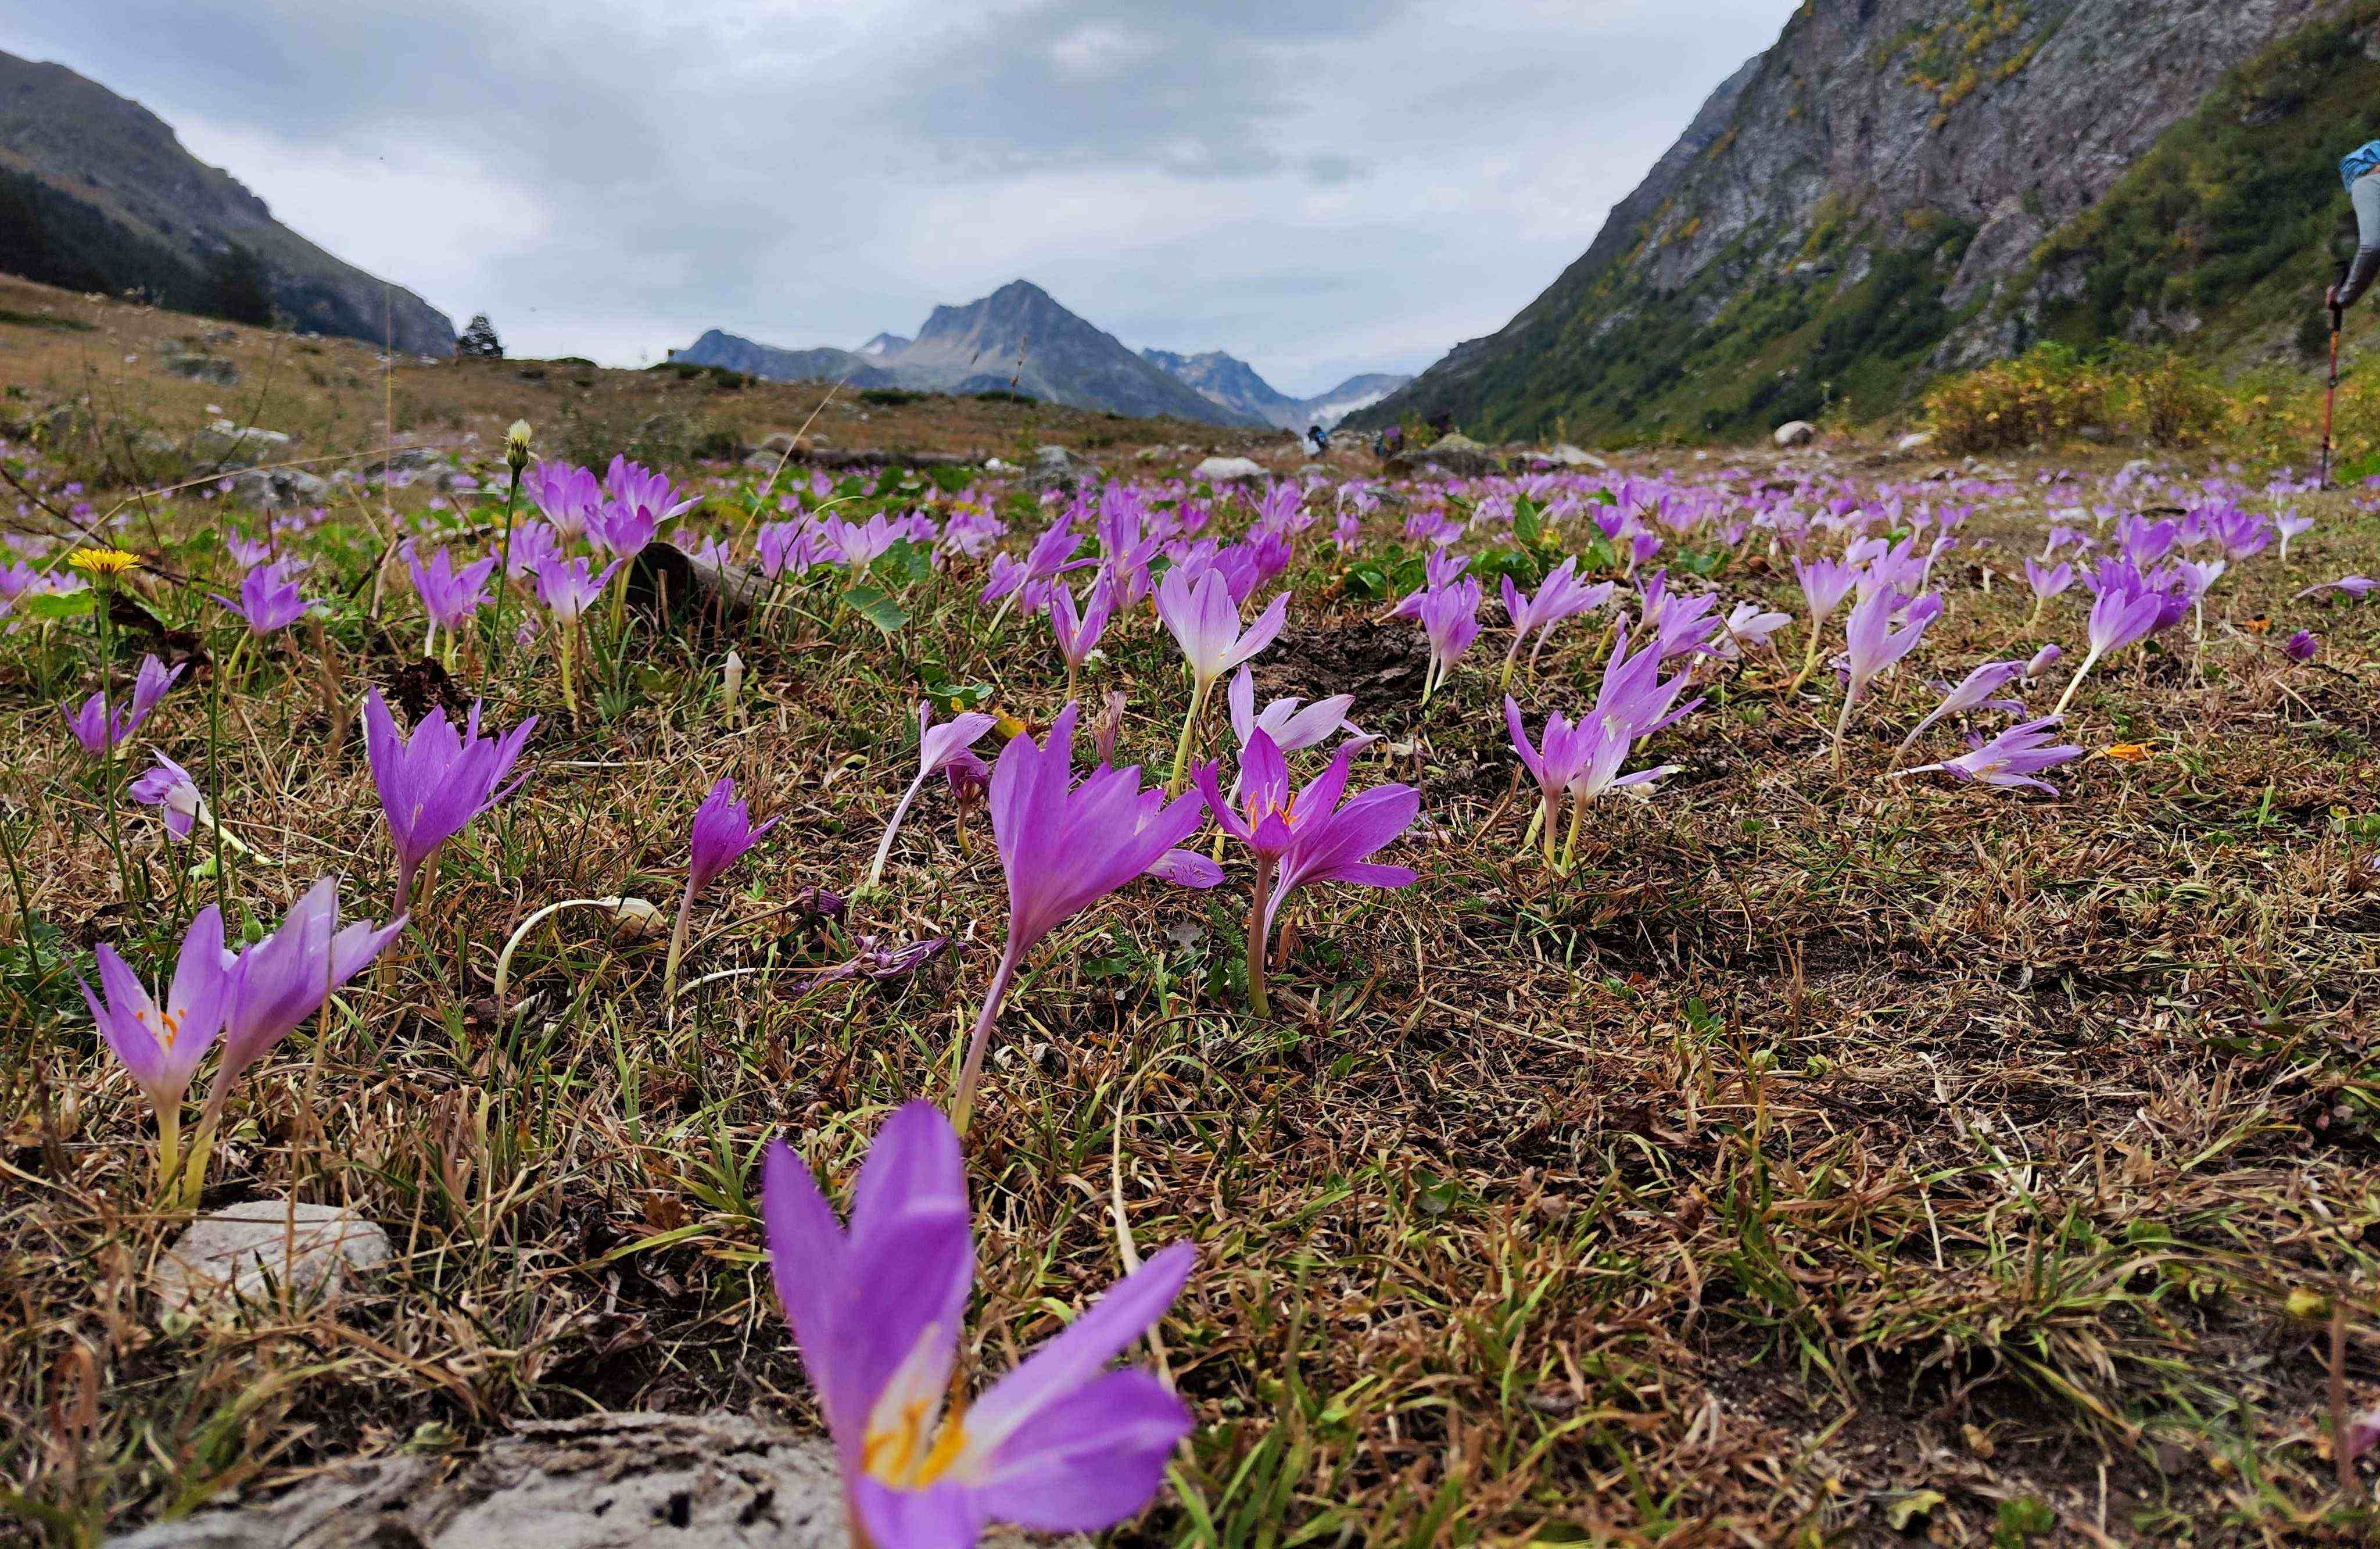
\includegraphics[width=0.7\linewidth]{../pics/IMG_20240822_101505}
	\caption{Крокусы в д.р. Джалпаккол}
	\label{fig:IMG_20240822_101505}
\end{figure}

В 11:45 дошли до развилки

\newpage